\section{Cross Modal Enhancement}

In this section, we introduce the Cross-Modal Enhancement and describe its role for video understanding tasks.

% \azsays {The following is too vague: here you need to give some idea of the modality-specific signals (e.g. speech, scene-text, faces) and very important - the time interval over which you are combining modalities (and creating the representation from), e.g. a video clip.}

\subsection{Resolving modality-specific ambiguities through filtering}

The objective of Cross-Modal Enhancement (CME) is to transform a collection of modality-specific video signals $\{\bm_i \}_{i \in \mathcal{M}}$ so as to render them maximally discriminative for a given task.  While these signals may be generic, the focus of this work is on high-level video understanding tasks, namely text-video retrieval and action recognition---consequently the set of signals under consideration include examples such as human speech and scene-text.  In the description that follows, we assume that that each such signal, $\bm_i$, takes the form of a fixed-size embedding (and therefore that temporal aggregation of each signal has been performed upstream).  The functional form of Cross-Modal Enhancement comprises a pair of functions: a \textit{filter generator}, $f_\phi$, the \textit{application function}, $a_\theta$, which are composed as follows:

\begin{align}
    \text{CME}(\bm_i) = a_\theta (\bm_i,  f_\phi (\{\bm_j: j \in \mathcal{N}_i\}))
    \label{eqn:cmf}
\end{align}

Here $\mathcal{N}_i$ denotes the \textit{filtering neighbourhood} of signal $\bm_i$, namely the signals which are used to generate its enhancement filter.  Cross-Modal Enhancement can thus be decomposed into its three components: (1) the selection of the filtering neighbours set, $\mathcal{N}_i$; (2) the choice of filter generator, $f_{\phi}$; (3) the design of the application function, $a_\theta$.  We discuss these choices below.

\subsubsection{Filtering Neighbourhoods:} A natural choice for the filtering neighbourhood of each input is simply the set of all signals (the filter sets therefore correspond to a dense graph, in which the signals are nodes and the edges define the neighbourhood inclusion relation).  Should prior knowledge about the relationships between the signals be available, it can be encoded directly into the filtering neighbours by imposing appropriate sparsity constrains on the inclusion graph.  In this work, we consider only small numbers of modality-specific signals and we therefore simply opt to use all possible nodes for each filtering neighbourhood, deferring further investigations of graph structure for large numbers of signals to future work.  Nevertheless, note that even dense inclusion graphs can be made computationally tractable with the appropriate choice of filter generator function---we describe this design choice next.


\begin{figure}[t]
\begin{center}
        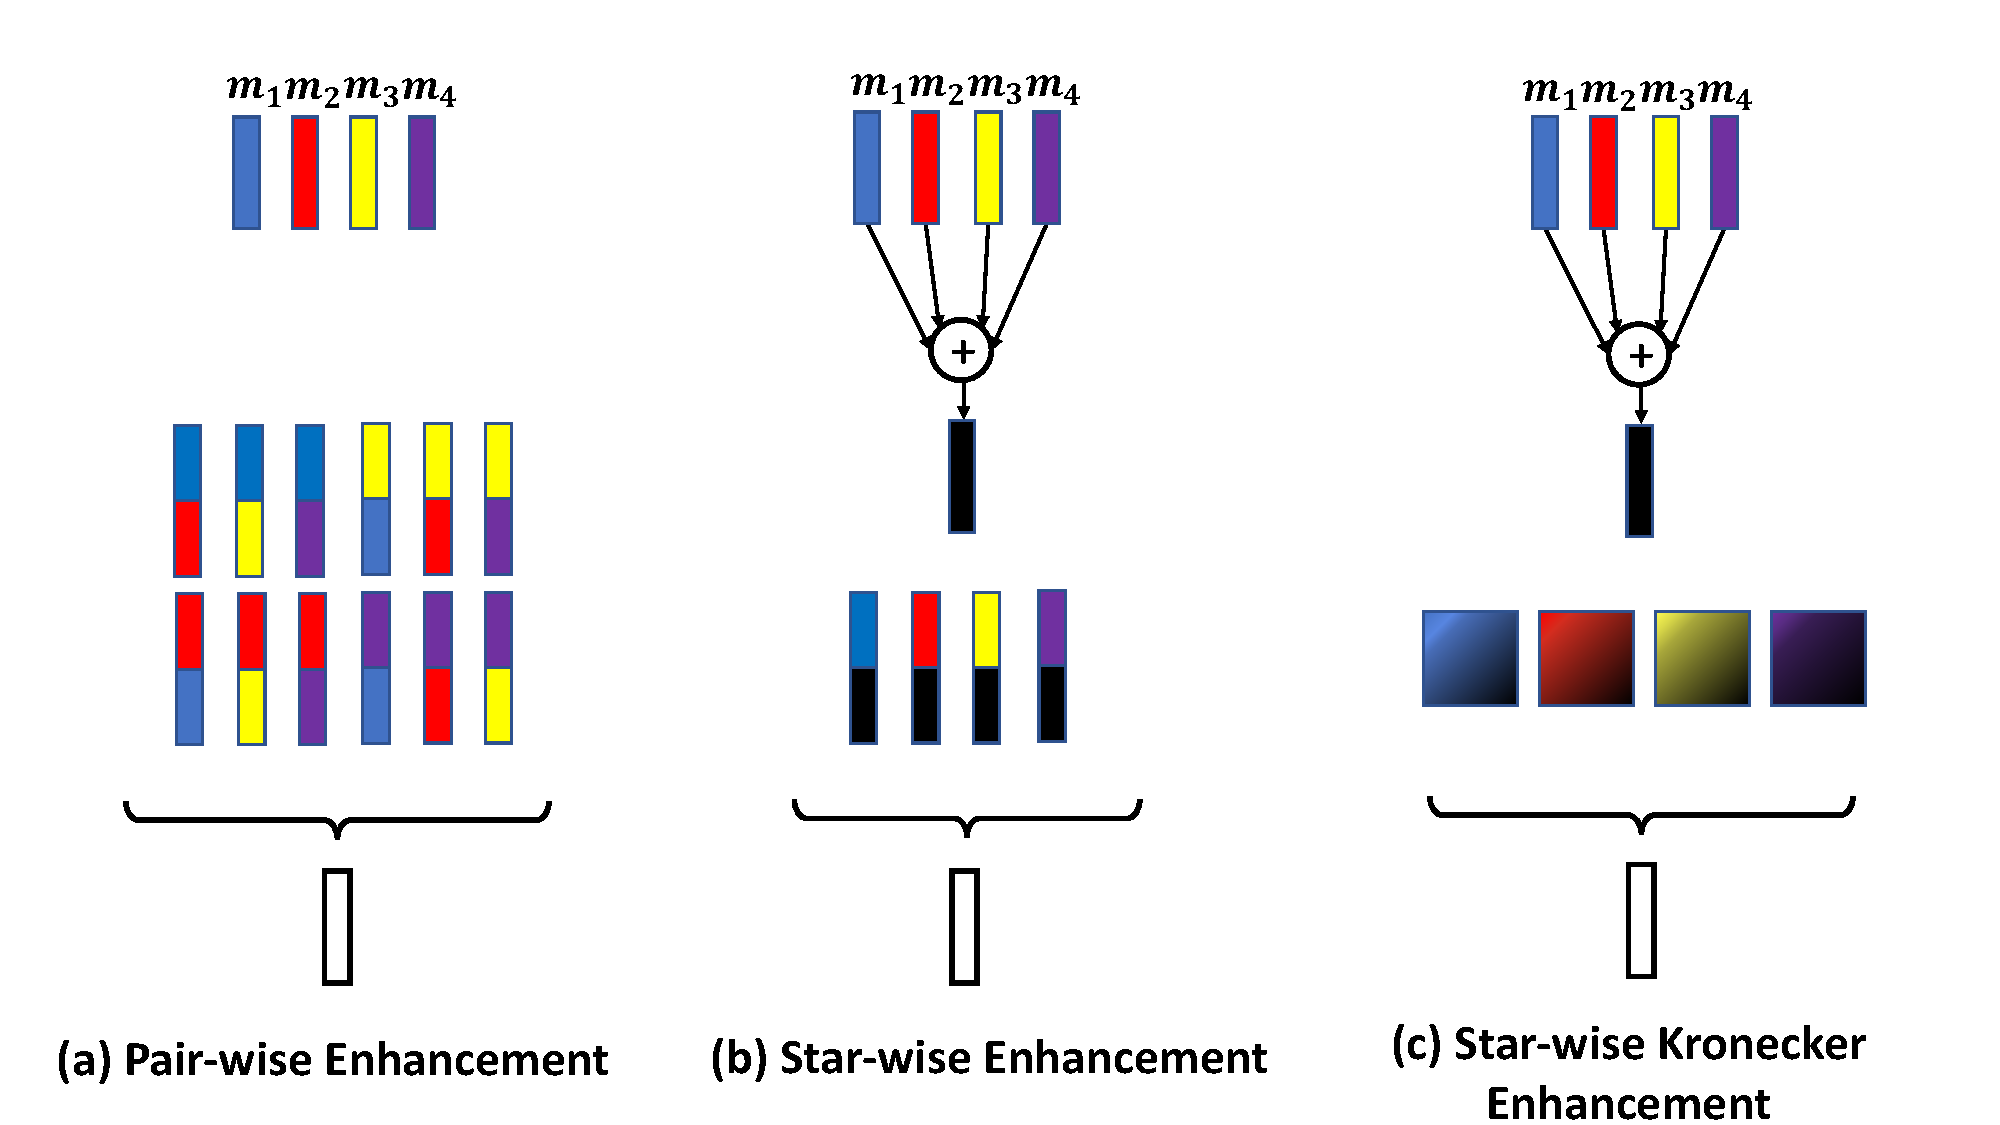
\includegraphics[scale=0.25]{filter_figure.pdf}
\end{center}
%\setlength{\abovecaptionskip}{-5pt}
%  \setlength{\belowcaptionskip}{-5pt}
\vspace{-4mm}
   \caption{Architecture} 
\label{fig_archi}
\vspace{-5mm}
\end{figure}
\subsubsection{The Filter Generator:} The objective of the filter generator, $f_\phi$, is to exploit the signal provided by the  neighbourhood $\mathcal{N}_i$ to produce a filter that maximally enhances the discriminative information for a given task. Intuitively, enhancement can be achieved through resolving ambiguity within a signal via reference to cues from its neighbours. It follows that to achieve this objective, the functional form of the generator should allow it to reason about the relationship between the contextual signal of the neighbourhood and the signal to be filtered.  To design such a generator, we draw inspiration from the Relation Network (RN) \cite{santoro2017simple}, and consider the following functional form for the filter generator:
\begin{equation} \label{pairwise} 
 f_\phi (\{\bm_j: j \in \mathcal{N}_i\}) = h_\phi (\sum_{j\neq i} g_\theta (m_i,m_j)),
\end{equation}
where functions $h_\phi$ and $g_\theta$ are used to model the pairwise relationship between signal $m_i$ and  $m_j$. More specifically, $g_\theta$ aims to aggregate structure information from each neighbour and $h_\phi$ combines the information from different sources. It dictates that the filter aims to learn and infer the existence and implication of all pair-wise signal relations within its filter field. 


However, the fully pairwise formulation typically contains many connections and parameters, which thus naturally brings redundancy in the connections, and also makes the network optimisation more difficult, particularly in the presence of limited training data. In order to substantially reduce the computational overhead of large fully-connected graphs, we modify the functional form described above.  Concretely, we propose to prune the set of relational pairs to the star topology imposed via Eqn.~\ref{star}.


% an intuition solution should be reducing the filter receptive field. However in various machine learning tasks, learning deep representations capturing both local and global receptive fields is important for the model performance [37, 35]. To maintain a large filter receptive field while utilising much fewer parameters than the fully-connected setting,  

\begin{equation} \label{star} 
 f_\phi (\{\bm_j: j \in \mathcal{N}_i\}) = h_\phi (g_\theta (m_i,\sum_{j} m_j)),
\end{equation}

This function combines a single pooling operator over all neighbours within the filter field to first obtain the context vector representation. Then for each signal, only relations between the input with the context vector are directly inferred. Such an approach encourages greater generalisation for computing relations, since $g_\theta$ is encouraged to not over-fit to the features of any particular signal. In contrast to the quadratic computational complexity pairwise topology implied by Eqn.~\ref{eqn:cmf}, the cost of a forward pass through the star-topology scales linearly with the number of inputs (see Fig.~\ref{fig_archi} centre). It is also worth noting that the star topology the summation in Eqn.~\ref{star} also ensures that the filter is invariant to the order of objects in the input signal. This invariance ensures that the filter output contains information that is generally representative of the relations that exist in the signal set.
 
While Eqn.~\ref{star} brings computational efficiency, it comes at a cost.  In essence, by exchanging the ordering of the summation over signals and $g_\theta$, the functional form of the filter generator no longer forms a natural for the pairwise interactions amongst the inputs.  In order to preserve the effective modelling capacity of the generator, whilst at the same time maintaining its attractive linear scaling, we therefore look to \textit{approximate} the the set of interactions directly in feature space.  We perform this approximation via a tensor product between the context vector and the incoming filter.  Intuitively, the tensor product offers a simple mechanism for  modelling interactions between feature sets \cite{long2017deep}, since each feature in the tensor product space corresponds to the product of a pair of features in the original feature set. Prior work has shown that this approximation of the statistics of the joint feature representations between two features \cite{song2013robust} is reasonable, given appropriate sample sizes. In more detail, we perform the tensor product between the $i^{(th)}$ modality signal $m_i$ and the context vector $\sum_{j} m_j$ when forming the input to function $g_\theta$, providing additional information in comparison to direct feature concatenation.  However, for even moderately sized input signals, the use a tensor product $m_i \otimes \sum_{j} m_j$ would be prohibitively expensive in both computation and memory.  We therefore opt to first project both operands of the tensor product to a lower dimension via a learnable linear projection $g_\theta$, prior to performing the tensor product:

\begin{equation} \label{star} 
 f_\phi (\{\bm_j: j \in \mathcal{N}_i\}) = h_\phi (g_\theta (m_i) \otimes g_\theta (\sum_{j} m_j)),
\end{equation}

% @Yang, I don't understand what this means.... :)
% Another tight approximation of the original  Eq ~(\ref{pairwise}) is calculating the tensor product between each single signal with the context vector. Assuming we have two vector spaces $V$ and $U$, their tensor product $V \otimes U$ intuitively is the idea "for each vector $v \in V$ ", attach it the entire vector space $U$.
% To obtain  $V \otimes U$, we start from the product space $U \times V$ and consider the free abelian group oover it denoted by $\mathcal{F}(U \times V)$. Given this larger space, that admits scalar products of ordered pairs, we we set up equicalence relations of the form $(av, u) a(v, u) (v,au) $ with $u \in U$, $v \in V$ and $a in \mathcal{F}$(a field) so that we identify points in the product space that yield multi-linear relationships in the quotient space generated by these relationships.

% \begin{itemize}

%     \item Pairwise CE.  Used in prior work.  Inspired by the Relation Network \cite{santoro2017simple}
%     \item The star topology
%     \item The Kronecker product approximation to the joint distribution.
%     % \item The triplet topology
% \end{itemize}
\subsubsection{Application Function:} Finally, we consider the choice of application function $a_\theta$.  While many choices are possible here, we follow prior work  successful designs of attention mechanism for feature enhancement (e.g. \cite{dauphin2017language,hu2019squeeze}) which apply a sigmoid operator over the generated filter to produce a $[0, 1]$-normalised mask. This mask is then multiplied element-wise back through the original signal.

% \textbf{Relationship to Attention}: One interpretation of Cross-Modal Enhancement is as an attention mechanism operating between the incoming signals.    {Maybe we want to talk about the relationship with dynamic filter, Message passing neural networks, attention mechanisms, etc.}



% As the number of inputs grows, it may be desirable to impose sparsity on the inclusion graph 

% In the absence of prior knowledge indicating that the a sparse graph should be used, a natural choice for the filtering neighbourhood in 

% We first assume access to a collection of modality-specific feature extractors $\{ \Phi_m \}_{m \in \mathcal{M}}$.  These may operate at either the video-level, or in the case of visual models, at the frame-level.  For example, one such frame-level feature extractor operating on the visual modality could be a convolutional neural network whose parameters have been optimised for the task for image classification.  This model therefore transforms the raw pixel data present in each frame of a video into a single embedding.  We next assume access to a corresponding family of temporal aggregation functions $\{ T_m \}_{m \in \mathcal{M}}$, which transform, for each feature extractor, its outputs into a fixed size representation.  A temporal aggregation function may be heavily parameterised, or simply comprise a pooling operation such as max or sum pooling. 

% Given the above, our goal is to transform the temporally aggregated modality-specific feature extractors $\{T_m(\Phi_m(\mathbf{v})): m \in \mathcal{M}\}$ of the source video that compactly represents the content within it that is relevant for a given task.  There are many ways 

% We reason via a lightweight attention mechanims.  The core idea (CE).

% \subsection{Extension to higher order interactions}



% \subsection{AHOI: An Efficient Approximation to higher-order reasoning}
\\
The general nature of the CME design described above allow for its direct integration into architectures for video understanding.  We its investigate its application in two representative tasks: text-video retrieval and action recognition, described next.

\subsection{Text-Video Retrieval Model}

The task of text-video retrieval requires a system to rank a collection of videos according to how well they match a given text query.  Joint video-text embeddings (which seek to map videos and text descriptions into a common space such that matching video and text pairs are close together) form an attractive model for tackling this problem, since they readily allow for efficient indexing: compact video embeddings can be pre-computed and stored offline such that the test time query reduces to simple distance computation between embeddings.

To assess the proposed CME approach, we adopt as a backbone the MoEE/CENet joint text-video embedding architecture proposed by \cite{miech2018learning} and extended more recently by \cite{liu2019use}.  In particular, the CENet architecture represents the state-of-the-art on several popular retrieval benchmarks.  Moreover, it utilises a particular form of \textit{pairwise} filtering to combine different signals of different modalities, making it an ideal starting point for our investigations.   We first briefly summarise the model, then describe the integration of CME as a component of the architecture.

The MoEE/CENet architecture comprises two core elements: a video encoder and a text encoder, which are learned to map videos and text into a common space.  CENet derives its strong retrieval performance by composing together the embeddings of a diverse collection of ``experts'': these are machine perception models which have been pretrained for related tasks, but not directly for retrieval.  In particular, they use deep neural networks pretrained for classification on the ImageNet dataset~\cite{deng2009imagenet}, scene recognition on the Places dataset \cite{zhou2017places}, action recognition models pretrained on Kinetics~\cite{}


\subsection{Action Recognition Model}

\begin{figure*}
    \centering
    \includegraphics[width=\textwidth,height=2in]{example-image-a}
    \caption{\textbf{The family of filter generation functions considered in this work}.}
    \label{fig:reasoning}
\end{figure*}